\scanpage{40}
\margin{\handwritten{$\times$}}
où $X_2=(X_1,p_2)\mathbin{\mathrm{x}}_{X_o}(X_1,p_1)$ (cf. IV \handwritten{9} pour le procédé de recollement de topos par données de descente).

Lorsque les conditions précédentes sont satisfaites, on dira que le topos annelé $(E,\underline{O}_E)$ est une \uline{étendue algébrique}\deleted{\unsure{.}} (comparer avec la notion d'étendue topologique IV \handwritten{9.}).
\margin{\handwritten{$\times$}}

10.3. Montrer qu'une étendue algébrique a suffisamment de points.

\margin{\handwritten{$\times$}}
\unsure{\deleted{B}U|\deleted{U}B|\deleted{S}U|\deleted{U}S}ne étendue algébrique est \uline{localement} annelé\handwritten{e} (IV \handwritten{11.}), et si $E,E'$ sont deux étendues algébriques, la catégorie \uline{\deleted{\unsure{g|p}}Homtoplocan}$(E,E')$ (IV \handwritten{11.}) est un groupoïde (toute flêche est inversible). (Procéder pour le premier point comme dans IV \handwritten{9.}; pour le deuxième, utiliser IV \hspace{2em}.)
\margin{\handwritten{$\times\quad\times$}}

10.4. \inserted{\handwritten{(Comparer \uline{IV} 9.\hspace{1em}.)}}\figure{\begin{tikzpicture}[x=0.01cm,y=0.01cm]\draw (35,8) .. controls (25,37) and (34,45) .. (65,47) .. controls (170,53) and (405,42) .. (425,65);\end{tikzpicture}} Soit $E$ une étendue algébrique. Montrer que les conditions suivantes sont équivalentes:
\margin{\handwritten{$\times$}}

(i) Pour toute étendue algébrique $E'$, la catégorie \deleted{Homtop} \uline{Homtoplocan}$(E',E)$ est rigide, i.e. \deleted{c'est} (comme c'est un groupoïde) elle est équivalente à une catégorie discrète.

(ii) Même énoncé, $E'$ étant le topos ponctuel annelé par un corps algébriquement clos.En d'autres termes, pour tout point géométrique (IV \handwritten{\unsure{11b|61b|\deleted{8}10}}) de $E$, le groupe des automorphismes de $p$ est le groupe unité.
\margin{\handwritten{$\times$}}

(iii) (Lorsque $E$ est exprimé en termes d'une prérelation d'équivalence \inserted{étale}\figure{\begin{tikzpicture}[x=0.01cm,y=0.01cm]\draw (116,20) .. controls (112,48) and (127,56) .. (150,56) .. controls (180,55) and (211,55) .. (213,85);\end{tikzpicture}} $X_1$ dans un schéma $X_o$, comme dans 10.2 (iii).) La prérelation d'équ\unsure{\deleted{k}i|\deleted{i}k}valence $(X_1,p_1,p_{2_{\deleted{\unsure{2|0}}}})$ dans le schéma $X_o$ est une relation d'équ\unsure{\deleted{k}i|\deleted{i}k}valence, i.e. le morphisme $(p_1,p_2):X_1\handwritten{\longrightarrow}X_o\mathbin{\mathrm{x}}X_o$ est un monomorp\unsure{\deleted{y}h|\deleted{h}y|\deleted{g}h|\deleted{m}h|\deleted{h}h}\unsure{\deleted{ç}i|\deleted{i}ç|\deleted{j}i|\deleted{i}i}sme.

Lorsque ces conditions sont satisfaites, on dit que l'étendue algébrique $E$ est \uline{rigide}, ou encore que $E$ est un \uline{espace} \uline{algébrique} \handwritten{(*)}

10.5.
\figure{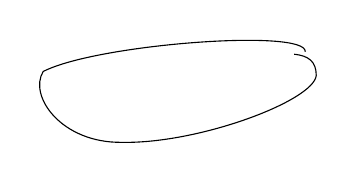
\begin{tikzpicture}[x=0.01cm,y=0.01cm]\draw (350,123) .. controls (353,153) and (85,133) .. (17,98) .. controls (-2,67) and (40,7) .. (117,8) .. controls (215,6) and (361,61) .. (364,93) .. controls (364,111) and (354,118) .. (336,120);\end{tikzpicture}}

\handwritten{(*) La terminologie est due à M. ARTIN, qui a mis en évidence l'importance de cette notion en Géométrie Algébrique.}
% archive sheet number: 39
